\documentclass{article}
\usepackage[utf8]{inputenc}
\usepackage[margin = 0.8in]{geometry}
\usepackage{graphicx}
\usepackage{amsmath, amssymb}
\usepackage{subcaption}
\usepackage{multirow}
\usepackage{mathtools}
\usepackage{float}
\usepackage{pythonhighlight}

\title{RBE549 - Homework 7}
\author{Keith Chester}
\date{Due date: November 1, 2022}

\begin{document}
\maketitle

\section*{Problem 1}

In this problem we are shown a number of shapes and then wish to find the $r(\theta)$ for the given shapes. The image below shows this:

\begin{figure}[H]
    \centering
    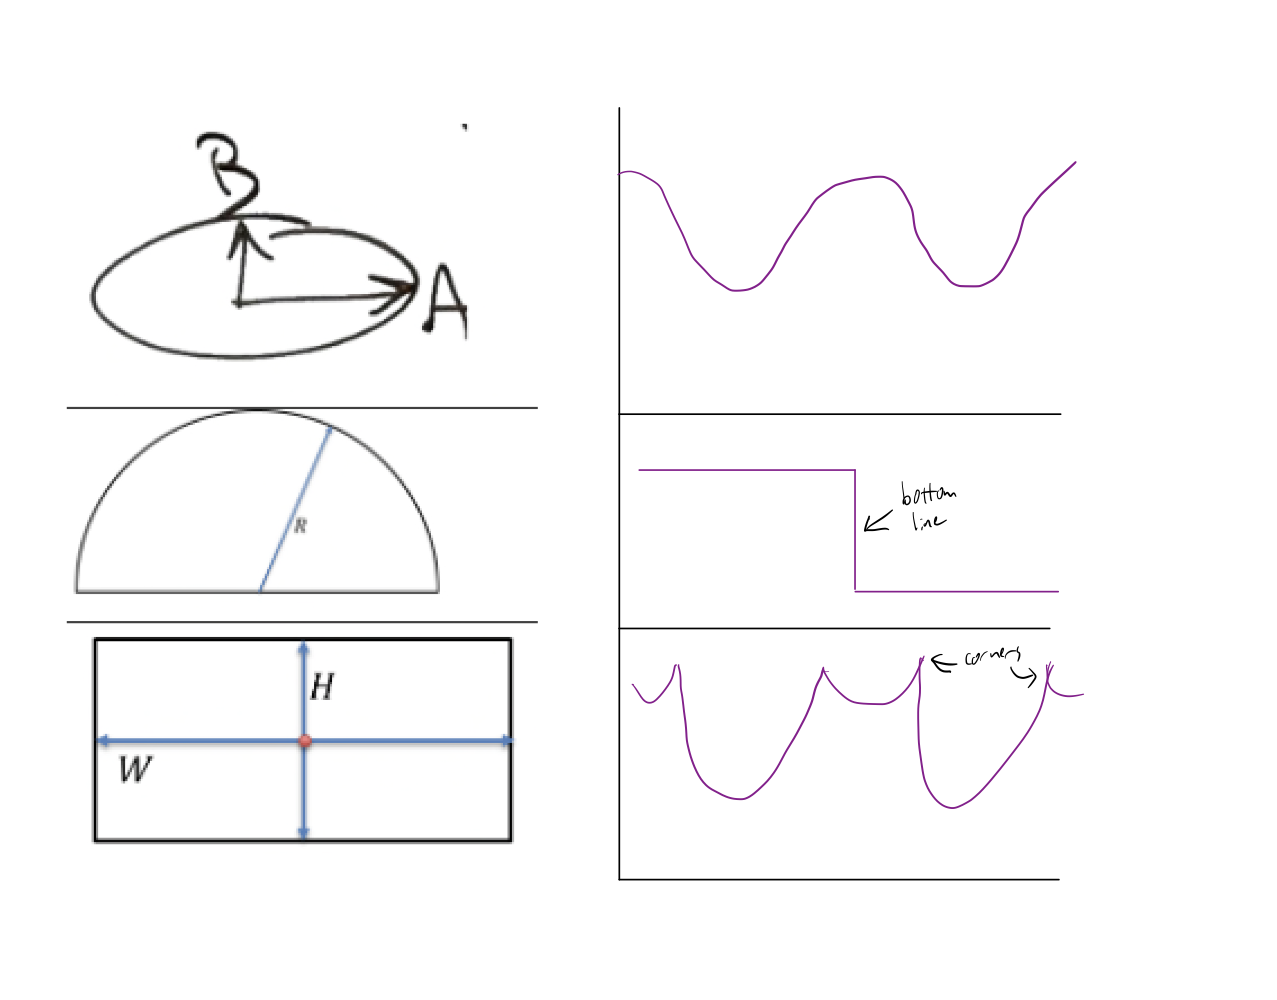
\includegraphics[width = 0.75\textwidth]{imgs/prob_1.png}
    \caption{$r(\theta)$}
    \label{fig:prob1-1}
\end{figure}

\section*{Problem 2}

In this problem we are aske a hypothetical problem. Supposing that we have a 2-class classification problem with centroid points $\mu A$ and $\mu B$, and that each classes are equally likely, we need to show that the Nearest Mean classifier decision boundary is midway along the line segment connecting $\mu A$ to $\mu B$.

First, we can look at the problem in $1$, $2$, and $3$ dimensions. For a $1D$ classifier, the resulting points would fall on a line and the resulting bounary would be between the centroids. If we looked at a $2D$ classifier, we would see the resulting decision boundary would be a line. Finally, for a $3D$ classifier, the decision boundary would be a plane. In each we depict the boundaries at a set distance $d$ between centroids.

\begin{figure}[H]
    \centering
    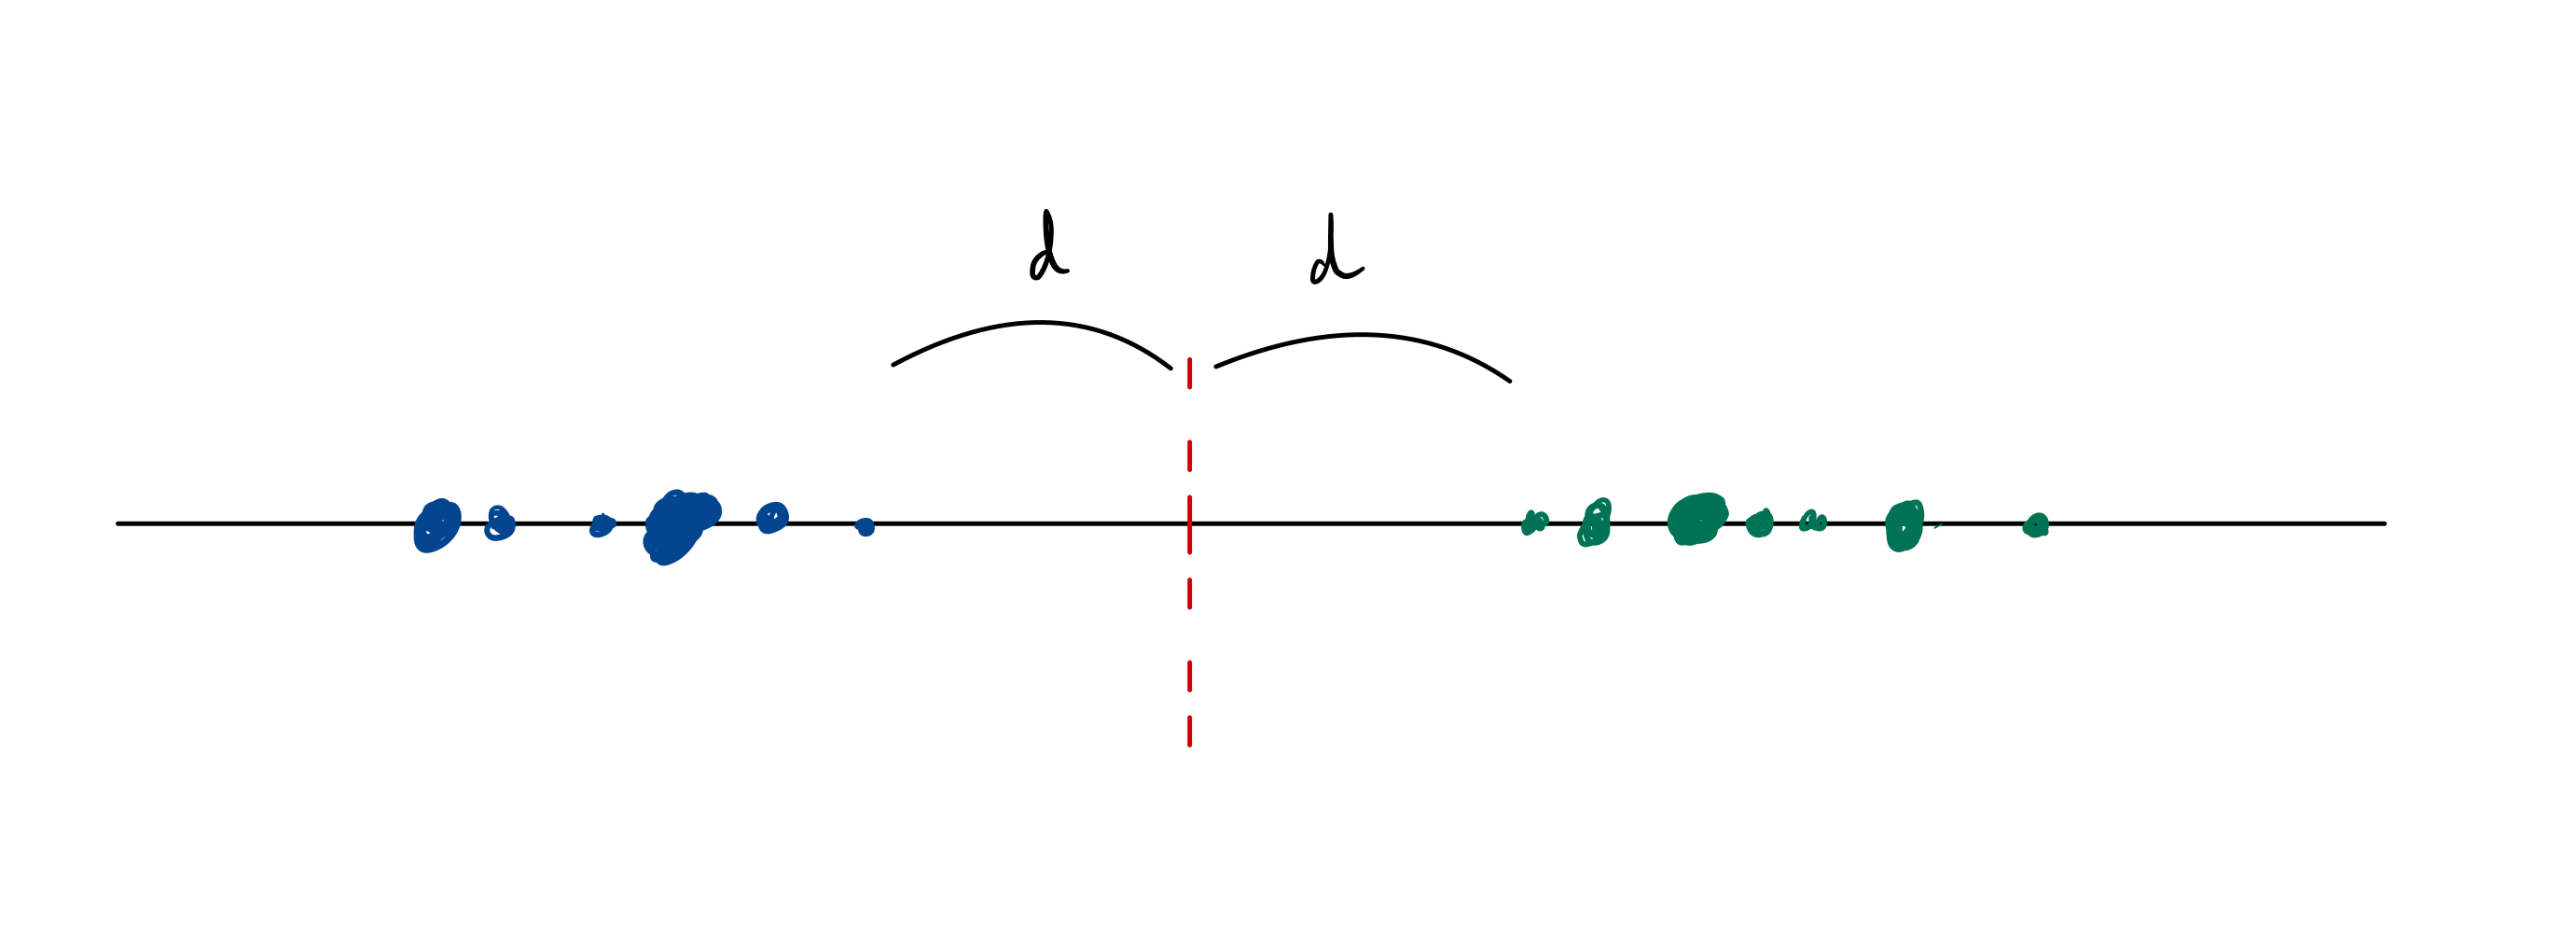
\includegraphics[width = 0.65\textwidth]{imgs/prob2_a.png}
    \caption{$1D$ Classifier}
    \label{fig:prob2-1}
\end{figure}

\begin{figure}[H]
    \centering
    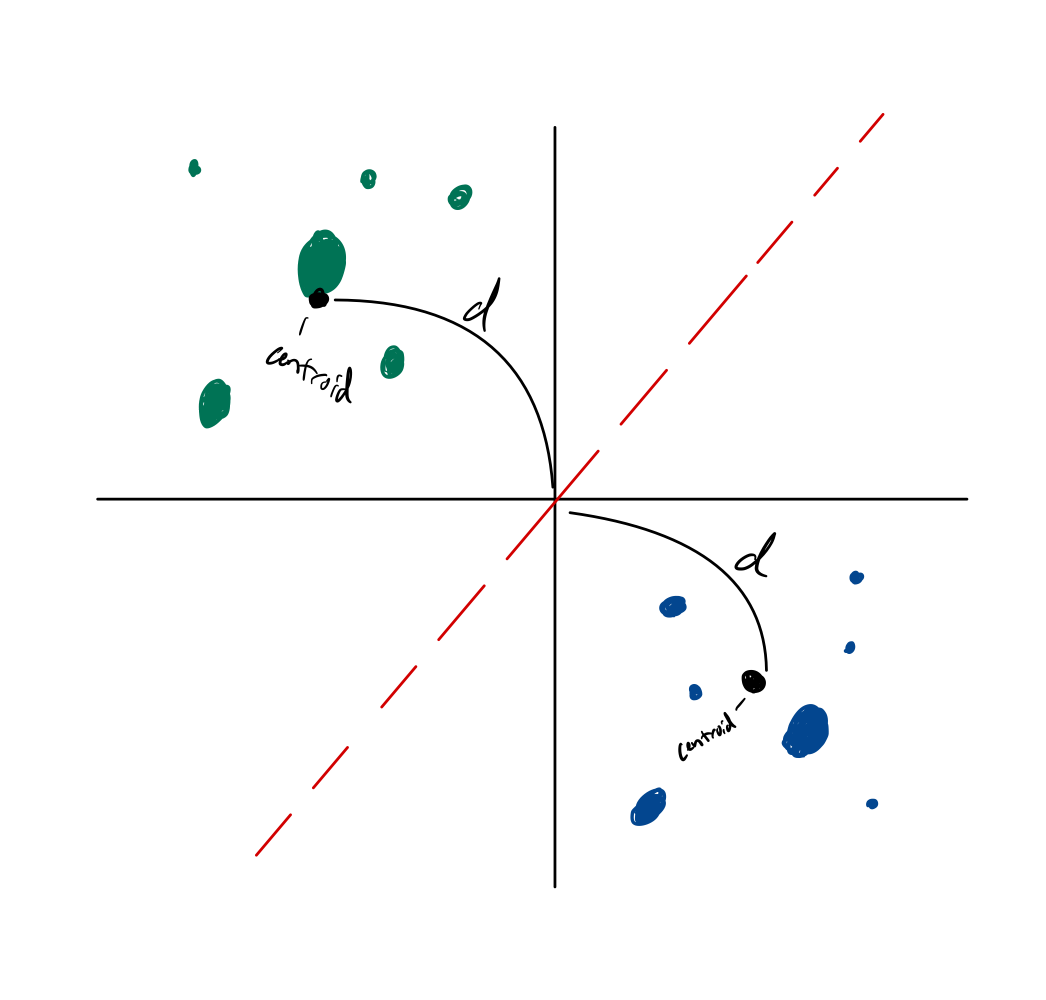
\includegraphics[width = 0.65\textwidth]{imgs/prob2_b.png}
    \caption{$1D$ Classifier}
    \label{fig:prob2-2}
\end{figure}

\begin{figure}[H]
    \centering
    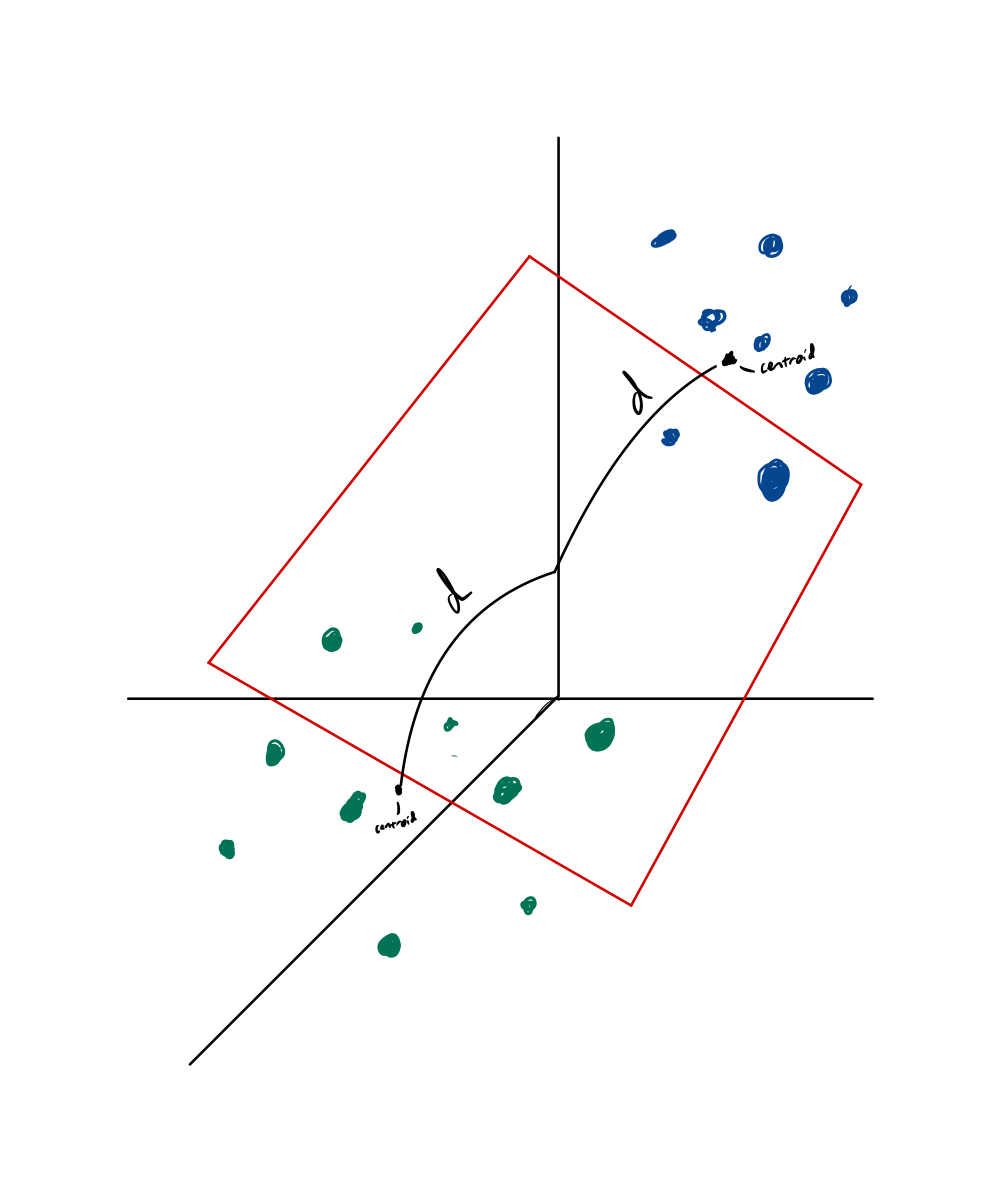
\includegraphics[width = 0.65\textwidth]{imgs/prob2_c.png}
    \caption{$3D$ Classifier}
    \label{fig:prob2-3}
\end{figure}

Since the problem states that the two classes $A$ and $B$ are equally likely, it means the the resulting centroids would be equidistant from a properly calculated Nearest Mean decision boundary. If either class had a higher probability than the other, the decision boundary as calculated via Nearest Mean would be closer to the centroid of that class.



\section*{Problem 3}

In this problem we are asked to represent an object by its boundary $(x(s),y(s)),0\leq s\leq S$ where $S$ is the length of the object's boundary and $s$ is distance along that bonudary from some arbitrary starting point. Combine $x$ and $y$ into a single complex function $z(a)=x(s)+jy(s)$. The Discrete Fourier Transform (DFT) of $z$ is:

\begin{equation}
    Z(k) = \sum^{S-1}_{s=0} e^{-2*\pi j \frac{ks}{S}} z(s), 0\leq k \leq S-1
\end{equation}

We can use the coefficients $Z(k)$ to represent the object boundary. The limit onf $s$ is $S-1$ because for a closed contour $Z(S)=z(0)$. The Inverse Discrete Fourier Transform is:

\begin{equation}
    z(s) = \frac{1}{S} \sum_{k=0}^{S-1} e^{+2\pi j \frac{ks}{S}} Z(k), 0 \leq s \leq S-1
\end{equation}

\subsection*{A}

Here we suppose that the object is translated by $(\Delta x, \Delta y)$, such that $z'(s) = z(s) + \Delta x + j \Delta y$. How is $z'$'s DFT $Z'(k)$ related to $Z(k)$? Stating again, that we start with:

\begin{equation}
    Z(k) = \sum^{S-1}_{s=0} e^{-2*\pi j \frac{ks}{S}} z(s), 0\leq k \leq S-1
\end{equation}

\noindent Which we can define $z'(s)$ as:

\begin{equation}
    z'(s) = z(s) + \Delta x + j \Delta y
\end{equation}

\noindent If we plug this into our original equation, we get...

\begin{equation}
    Z'(k) = \sum_{s=0}^{S-1} e^{-2\pi j \frac{ks}{S}}z(s) + \sum_{s=0}^{S-1} e^{-2\pi j \frac{ks}{S}} (\Delta x + j \Delta y) (1)
\end{equation}

\noindent Here we see that we have a segment that is equivalent to oru defined $Z(k)$, so we can simplify by expressing:

\begin{equation}
    Z(k) + (1) (\Delta x + j \Delta y) \sum_{s=0}^{S-1} e^{-2\pi j \frac{ks}{S}}
\end{equation}

\noindent With $\Delta x$ and $j \Delta y$ isolated, we can use a table of known Fourier Transforms to identify the resulting conversion. Based on our problem's definition $\Delta X$ and $\Delta y$ are both constants, so we can state that:

\begin{equation}
    Z'(k) = Z(k) + (\Delta x + j \Delta y) \sigma(\frac{2 \pi k}{S})
\end{equation}

\noindent ...where $\frac{1}{S}$ acts as our scaling factor.

\subsection*{B}

What object has $z(s) = R \cos(\frac{2\pi s}{S}) + jR \sin(\frac{4\pi s}{S})$? Below we see a graph drawing the shape, and included code to generate it. Random values were chosen for the $S$ and $r$ for the sake of plotting it.

\begin{figure}[H]
    \centering
    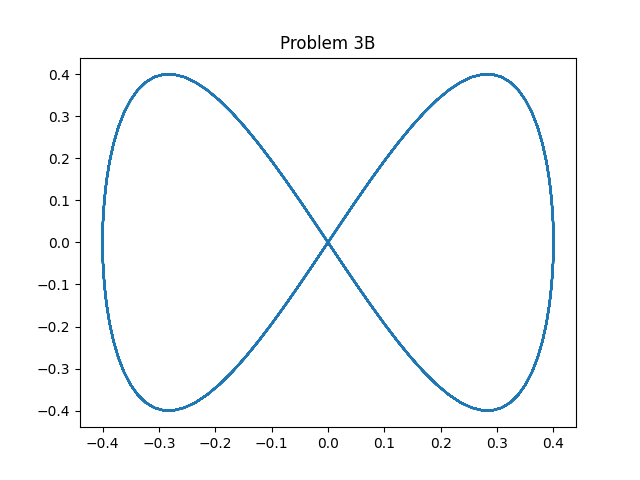
\includegraphics[width = 0.65\textwidth]{imgs/prob3_b.png}
    \caption{Our resulting shape}
    \label{fig:prob3-b}
\end{figure}

\begin{python}
import numpy as np
from numpy import cos, sin, pi
import matplotlib.pyplot as plt

figure = plt.figure()
plt.title("Problem 3B")

S = 10
r = 4

theta = [theta for theta in np.arange(0, S, 0.01)]
X = [
        r * cos(2*pi*theta)/S
        for theta in theta
    ]
Y = [
        r * sin(4*pi*theta)/S
        for theta in theta
    ]

# Plot the results
plt.plot(X, Y)
plt.savefig("./imgs/prob3_b.png")
\end{python}

\subsection*{C}

In this problem we are tasked with showing what $Z(k)$ is corresponding to $z(s)$. We begin with our equation from $B$:

\begin{equation}
    z(s) = R \cos(\frac{2\pi s}{S}) + jR \sin(\frac{4\pi s}{S})
\end{equation}

\noindent We can utilize the inverse of Euler's formula; $\cos(x)=\frac{e^{ix}+e^{-ix}}{2}$ and $\sin(t) = \frac{e^{ix}-e^{-ix}}{2x}$. This allows us to expand our starting equation:

\begin{equation}
    z(s) = \frac{R(e^{j \frac{2 \pi s}{S}}+e^{-j \frac{2 \pi s}{S}})}{2} + \frac{R (e^{j \frac{4 \pi s}{S}} - e^{-j \frac{4 \pi s}{S}})}{2}
\end{equation}

\noindent We can then begin simplifying our equation by moving out constants ($\frac{R}{2}$) and repositioning terms:

\begin{equation}
    \frac{R}{2} (e^{j \frac{2 \pi s}{S}}+e^{-j \frac{2 \pi s}{S}} + e^{j \frac{4 \pi s}{S}} - e^{-j \frac{4 \pi s}{S}})
\end{equation}

Looking at the discrete fourier transform (DFT) from earlier in our problem, specifically, we can then begin to expand on this equation. Our starting equation is:

\begin{equation}
    Z(k) = \sum^{S-1}_{s=0} e^{-2*\pi j \frac{ks}{S}} z(s), 0\leq k \leq S-1
\end{equation}

\noindent ...which can lead us to:

\begin{equation}
    Z(k) = \sum^{S-1}_{s=0} e^{-2*\pi j \frac{ks}{S}} (\frac{R}{2} (e^{j \frac{2 \pi s}{S}}+e^{-j \frac{2 \pi s}{S}} + e^{j \frac{4 \pi s}{S}} - e^{-j \frac{4 \pi s}{S}}))
\end{equation}

\begin{equation}
    Z(k) = \frac{R}{2} \sum^{S-1}_{s=0} e^{-j 2 \pi (k-1)}{S} + e^{-j 2 \pi (k+1)}{S} + e^{-j 2 \pi (k-2)}{S} + e^{-j 2 \pi (k+2)}{S}
\end{equation}

\noindent We know from a Fourier Transform lookup table that $e^{j 2 \pi \omega x_0}$ transforms to $2 \pi \sigma(x - x_0) $, so applying this here:

\begin{equation}
    Z(k) = \sigma(2 \pi \frac{k-1}{S}) + \sigma(2 \pi \frac{k+1}{S}) + \sigma(2 \pi \frac{k-2}{S}) + \sigma(2 \pi \frac{k+2}{S})
\end{equation}



\end{document}